\chapter{\IfLanguageName{dutch}{Stand van zaken}{State of the art}}%
\label{ch:stand-van-zaken}



% Tip: Begin elk hoofdstuk met een paragraaf inleiding die beschrijft hoe
% dit hoofdstuk past binnen het geheel van de bachelorproef. Geef in het
% bijzonder aan wat de link is met het vorige en volgende hoofdstuk.

% Pas na deze inleidende paragraaf komt de eerste sectiehoofding.

De Securities and Exchange Commission (SEC) vereist dat institutionele vermogensbeheerders een kwartaalrapport indienen dat bekend staat als Form 13F als ze zeggenschap hebben over USD 100 miljoen of meer in sectie 13(f) effecten. Sectie 13(f) van de Securities Exchange Act van 1934 verplicht de openbaarmaking van effectenbezit door grote institutionele beleggers om de transparantie te vergroten. In 1975 implementeerde het Amerikaanse Congres deze bepaling om de toegankelijkheid van informatie over de investeringsactiviteiten van deze bedrijven te verbeteren. De bedoeling was om het vertrouwen van beleggers in de integriteit van de effectenmarkten in de Verenigde Staten te vergroten door middel van een openbaarmakingsprogramma \textcite{SECform13F2024}.
Melding 13F biedt een uitgebreid overzicht van de aandelenbeleggingen van S\&P 500 bedrijven en is een zeer belangrijk hulpmiddel voor analisten, onderzoekers en beleggers die inzicht willen verkrijgen in markttrends en de beleggingsbenaderingen van belangrijke marktspelers. Het onverwerkte tekstformaat waarin deze inzendingen worden aangeleverd, vormt echter een aanzienlijke belemmering voor effectieve gegevensextractie en -analyse, vooral voor inzendingen van voor 2013. Voor 2013 ontbrak het bij 13F-meldingen vaak aan standaardisatie en systematische opmaak, wat nu wel gebruikelijk is bij recentere aanmeldingen.
Kunstmatige intelligentie (AI) en Machine Learning (ML) technologieën hebben de extractie en organisatie van gegevens uit ongestructureerde tekst de afgelopen jaren aanzienlijk veranderd. Geavanceerde methodologieën zoals Natural Language Processing (NLP) en Deep Learning (DL) modellen vergemakkelijken de omzetting van tekstuele 13F-meldingen in gestructureerde datasets die geschikt zijn voor grondige analyse en studie. Standaardisatie is cruciaal voor historische gegevens, omdat het ontbreken van uniformiteit geautomatiseerde verwerking kan bemoeilijken. Door gebruik te maken van deze technologieën kunnen zowel huidige als oudere 13F-meldingen worden omgezet in georganiseerde gegevens, die vervolgens kunnen worden opgeslagen in databanken, waardoor patronen eenvoudiger kunnen worden opgehaald, gevisualiseerd en geanalyseerd.

Het doel van deze literatuurstudie is het onderzoeken en beoordelen van de verschillende Artificial Intelligence (AI) en Machine Learning (ML) technieken die kunnen worden gebruikt om gegevens uit 13F-meldingen van voor 2013 te extraheren, te organiseren en op te slaan. Het doel van het onderzoek is het bepalen van de meest efficiënte methoden om de ongeorganiseerde inhoud van deze documenten om te zetten in een gestructureerd formaat dat geschikt is voor analyse en opslag in een database. Dit houdt in dat er een onderzoek wordt gedaan naar verschillende kunstmatige intelligentie methodologieën, zoals Natural Language Processing (NLP) en Text mining, en dat bepaalde tools zoals NLTK en SpaCy worden geëvalueerd. De literatuurstudie zal ook de integratie van gestructureerde gegevens in een Database Management System (DBMS) onderzoeken, om te garanderen dat de geëxtraheerde gegevens gemakkelijk beschikbaar zijn voor later onderzoek en analyse. Het doel van deze evaluatie is om een uitgebreide kennis te krijgen van de meest effectieve procedures en technologie voor het verwerken van 13F-meldingen. 
\section{Achtergrond informatie}
\subsection{Reden voor 13F-meldingen}
TODO
\subsection{Andere filings}
Naast de 13F filings zijn er verschillende andere belangrijke SEC-filings die investeringsbedrijven systematisch moeten indienen en die nuttig kunnen zijn voor het opbouwen van een eigen investeringsportfolio. Hier zijn enkele van de meest relevante:

\paragraph{Form 10-K}
De 10-K is een jaarlijkse rapportage die een uitgebreid overzicht biedt van de prestaties van een bedrijf gedurende het afgelopen jaar. Deze filing bevat gedetailleerde financiële gegevens, informatie over bedrijfsactiviteiten, risicofactoren en managementanalyses. Het is een cruciaal document voor investeerders die inzicht willen krijgen in de financiële gezondheid en strategie van een bedrijf \autocite{SECfiling2024} .

\paragraph{Form 10-Q}
De 10-Q is een kwartaalrapportage die bedrijven verplicht zijn in te dienen. Het biedt een update over de financiële prestaties en operationele activiteiten van het bedrijf in de afgelopen drie maanden. Dit document is minder uitgebreid dan de 10-K, maar biedt toch waardevolle informatie over de recente ontwikkelingen en trends  \autocite{SECfiling2024} \autocite{Baker2022}.

\paragraph{Form 8-K}
De 8-K is een actuele rapportage die bedrijven moeten indienen wanneer er belangrijke gebeurtenissen plaatsvinden die van invloed kunnen zijn op de aandelenprijs of de operationele status van het bedrijf. Dit kan bijvoorbeeld gaan om fusies, overnames, wijzigingen in het management of andere significante gebeurtenissen. Het is belangrijk voor investeerders om deze filings te volgen, omdat ze snel inzicht geven in belangrijke veranderingen binnen een bedrijf  \autocite{SECfiling2024}\autocite{CFI2024} \autocite{Baker2022}.

\paragraph{Roxy Statement (DEF 14A)}
De Proxy Statement bevat informatie over de jaarlijkse aandeelhoudersvergadering, inclusief details over stemprocedures, bestuursleden, en compensatie van het management. Dit document is waardevol voor investeerders die geïnteresseerd zijn in corporate governance en de belangen van aandeelhouders  \autocite{SECfiling2024} \autocite{Baker2022}.

\paragraph{Schedule 13D}
Schedule 13D moet worden ingediend door elke persoon of entiteit die meer dan 5\% van de aandelen van een publiek bedrijf aanschaft. Dit document bevat de identiteit van de aandeelhouder en de redenen voor de aankoop, wat nuttig kan zijn voor investeerders die de bewegingen van grote aandeelhouders willen volgen \autocite{CFI2024} \autocite{Baker2022}.

\paragraph{Form D}
Form D wordt gebruikt voor het melden van een privéplaatsing van effecten. Dit document kan nuttig zijn voor investeerders die geïnteresseerd zijn in alternatieve investeringsmogelijkheden of startups die kapitaal aantrekken zonder een volledige openbare aanbieding te doen  \autocite{SECfiling2024}.

Door deze verschillende SEC-filings te analyseren, kunnen investeerders een beter begrip krijgen van de bedrijven waarin ze geïnteresseerd zijn en weloverwogen beslissingen nemen bij het opbouwen van hun investeringsportefeuille.

% ----------------------------------------------------------------------------
\section{Wat zijn 13F-meldingen}

Het doel van deze sectie is om een beknopte inleiding te geven aan 13F-meldingen, met bijzondere aandacht voor de structuur van deze meldingen, de informatie die ze bevatten en de reden van hun bestaan.


\subsection{Definitie en doel}
Volgens \autocite{SECform13F2024} zijn 13F-meldingen verplichte wettelijke documenten die de Amerikaanse Securities and Exchange Commission (SEC) vereist onder Sectie 13(f) van de Securities Exchange Act van 1934. Deze deponeringen worden gebruikt om de portefeuilles van institutionele beleggingsbeheerders te rapporteren.

Het belangrijkste doel van 13F-meldingen is om duidelijkheid en openheid te bieden over de beleggingsactiviteiten van belangrijke institutionele beleggers. Deze vereiste vergemakkelijkt het toezicht op beleggingsposities van verschillende instellingen, zoals beleggingsfondsen, pensioenfondsen en andere belangrijke beleggingsbeheerders, door het publiek en regelgevende instanties.

\subsection{Belangrijke kenmerken}
Het doel van dit deel is het bespreken van enkele kenmerken van de 13F-meldigen waaronder wie het moet indienen en wat ze moeten inhouden.


\subsubsection{Vereisten voor rapportage:}

Institutionele beleggingsbeheerders die minimaal USD 100 miljoen aan beheerd vermogen beheren, zijn verplicht om elk kwartaal een 13F-melding in te dienen. Deze rapporten moeten gedetailleerde informatie bevatten over de aandelenportefeuille van de instelling. Dit omvat onder andere de naam van het aandeel, het CUSIP-nummer, het aantal aandelen dat wordt gehouden, en de marktwaarde ervan. 
\paragraph{CUSIP}
Volgens \autocite{Hayes_2024} is CUSIP een afkorting voor "Committee on Uniform Security Identification Procedures". Het is een comité binnen de American Bankers Association (ABA) dat een systeem heeft ontwikkeld voor het identificeren van Amerikaanse en Canadese effecten.

Een CUSIP-nummer is een uniek nummer bestaande uit 9 cijfers en letters dat aan elk effect wordt toegekend. Ze bieden een gestandaardiseerde methode voor het identificeren van effecten om de clearing en afwikkeling van transacties op de handelsmarkt te vergemakkelijken. Deze nummers werden beheerd door Standard \& Poor's maar FactSet Research Systems heeft dit overgekocht in naam van American Bankers Association(ABA) in 2022 zij beheren deze nummer nu ook \autocite{Hayes_2024}.

De CUSIP-code is een voorbeeld van een National Securities Identifying Number, een standaard identificatiemethode voor effecten.

\subsubsection{Omvang van de informatie:}

De rapportages over het aandelenbezit van grote beleggingsinstellingen richten zich voornamelijk op aandelen, terwijl andere soorten activa, zoals obligaties, derivaten en private equity, buiten beschouwing worden gelaten \autocite{SECform13F2024}. Elk kwartaalrapport biedt een beknopt overzicht van de aandelenportefeuille van de instelling aan het einde van de rapportageperiode. Dit overzicht geeft waardevolle inzichten in de investeringsstrategieën en methoden die de instelling hanteert, wat bijdraagt aan de transparantie en begrip van hun beleggingsbenadering.


\subsubsection{Opmaak en toegankelijkheid:}
De 13F-meldingen van voor 2013 zijn variërend in opmaak, dit is wat data extractie moeilijk maakt
Dit zijn enkele afbeeldingen van enkele van de tienduizenden 13F-meldingen

\paragraph{Voor 2013}
Hieronder zijn een aantal voorbeelden van de informatie tabel van enkele 13F-meldigen zichtbaar. Zoals te zien is, zijn er veel verschillende manieren waarop deze meldingen zijn ingediend.

\begin{figure}[hbt!]
    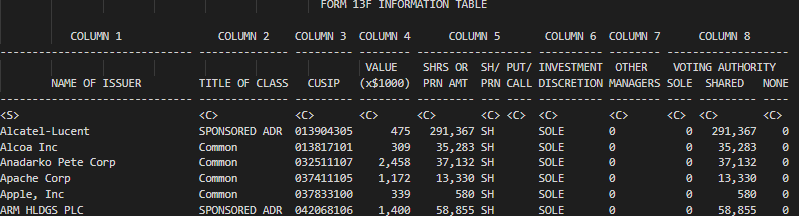
\includegraphics[width=0.8\textwidth]{13F_EX0.png}
    \caption[13F voorbeeld 1]{\label{fig:voorbeeld 1}Een correcte 13F-melding duidelijk gestructureerd en geen missende waarden}
\end{figure}


\begin{figure}[hbt!]
    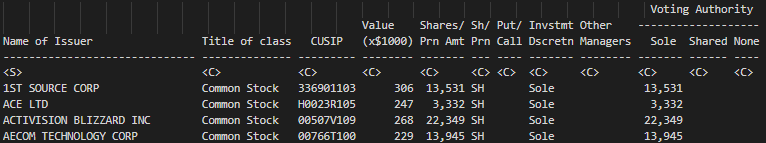
\includegraphics[width=0.8\textwidth]{13F_EX2.png}
    \caption[13F voorbeeld 3]{\label{fig:voorbeeld 2}Een 13F-melding met missende waarden}
\end{figure}
\begin{figure}[hbt!]
    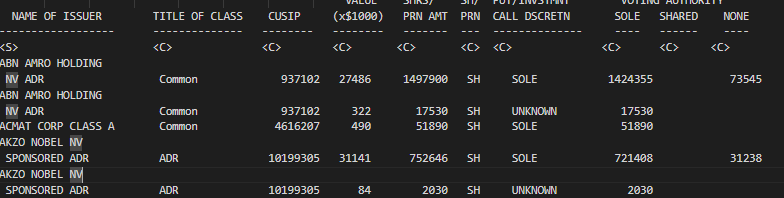
\includegraphics[width=0.8\textwidth]{13F_EX3.png}
    \caption[13F voorbeeld 4]{\label{fig:voorbeeld 3}Een 13F-melding met missende waarden en één entry overspant minstens één rij}
\end{figure}

\begin{figure}[hbt!]
    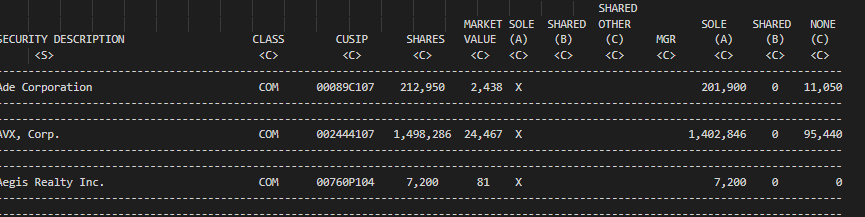
\includegraphics[width=0.8\textwidth]{13F_EX4.png}
    \caption[13F voorbeeld 5]{\label{fig:voorbeeld 4}Een 13F-melding gebruik makend van `X` in plaats van Bv. Sole}
\end{figure}

\begin{figure}[hbt!]
    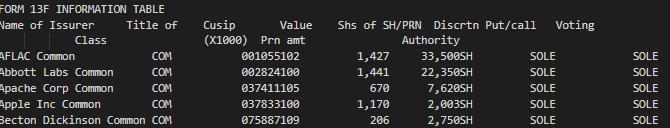
\includegraphics[width=0.8\textwidth]{13F_EX5.png}
    \caption[13F voorbeeld 6]{\label{fig:voorbeeld 5}Een 13F-melding zonder cijfer datas in de laatste kolommen}
\end{figure}

\begin{figure}[hbt!]
    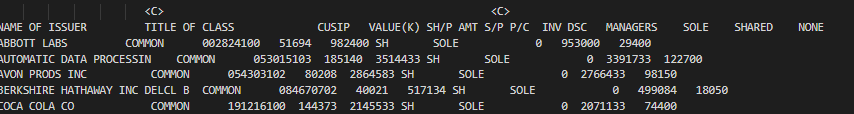
\includegraphics[width=0.8\textwidth]{13F_EX6.png}
    \caption[13F voorbeeld 7]{\label{fig:voorbeeld 6}Een 13F-melding zonder gestructureerde data maar werkend met tabs, geen tabel structuur}
\end{figure}
\paragraph{Na 2013}

\begin{figure}[hbt!]
    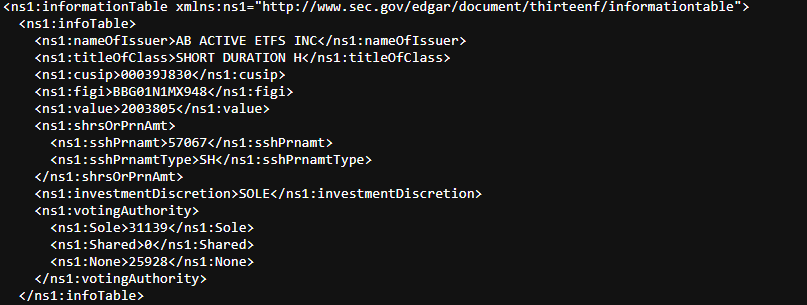
\includegraphics[width=0.8\textwidth]{13F_24_EX1.png}
    \caption[13F voorbeeld 7]{\label{fig:voorbeeld 2024 1}Een recente (2024) 13F-melding gestructureerd in XML}
\end{figure}
% ----------------------------------------------------------------------------


\section{Text mining en gerelateerde technieken}
Text mining, of ook bekend tekstdatamining, is de procedure om ongestructureerde tekst om te zetten in een gestructureerd formaat om significante patronen te ontdekken en nieuwe inzichten te verwerven \autocite{IBM2024}. Text mining maakt de analyse van uitgebreide tekstdatasets mogelijk om significante thema's, patronen en verborgen verbanden bloot te leggen. Deze techniek is essentieel voor het omzetten van ongestructureerde gegevens in gestructureerde gegevens, die vervolgens kunnen worden gebruikt voor analyse en besluitvorming.

\subsection{Document datatypes}
Volgens \autocite{AWS2024} kan text mining kan verschillende soorten gestructureerde gegevens omvatten, waaronder:

\begin{enumerate}
    \item \textbf{Gestructureerde Gegevens}: Deze gegevens worden in tabelvorm gebracht, wat het opslaan en verwerken voor analyse en machine learning-algoritmen vergemakkelijkt. Voorbeelden includeren databanken met kolommen en rijen.
    \item \textbf{Ongestructureerde Gegevens}: Deze gegevens hebben geen vooraf gedefinieerd formaat en kunnen tekst uit bronnen zoals sociale media of productrecensies bevatten, evenals rijke media zoals video- en audiobestanden. Aangezien financiële documenten vaak in ongestructureerd formaat bestaan, is text mining essentieel om deze gegevens om te zetten in een bruikbaar formaat.
    \item \textbf{Semi-gestructureerde Gegevens}: Deze gegevens vormen een mix tussen gestructureerde en ongestructureerde formaten. Ze hebben enige organisatie, maar voldoen niet volledig aan de vereisten van een relationele database. Voorbeelden hiervan zijn XML, JSON en Html-bestanden.
\end{enumerate}

Dit onderscheid zijn van groot belang voor het begrijpen van hoe text mining toegepast kan worden over de verschillende datastructuren, dit opent de mogelijkheid om de data de extraheren en belangrijke inzichten te verwerven.

\subsection{Text mining versus Text analytics}
Hoewel text mining en text analytics vaak door elkaar worden gebruikt, kan er een genuanceerd onderscheid tussen de twee gemaakt worden. Bij text mining gaat het meestal om het identificeren van patronen en trends in ongestructureerde gegevens, terwijl text analytics gericht is op het afleiden van kwantitatieve inzichten door gegevens op een gestructureerde manier te analyseren. Deze observaties kunnen vervolgens grafisch worden weergegeven om de ontdekkingen effectief over te brengen aan een breder publiek.\autocite{IBM2024}
\subsubsection{Text mining: vinden van verstopte patronen}
Text mining omvat het extraheren van waardevolle informatie en het identificeren van verborgen patronen uit uitgebreide verzamelingen ongeorganiseerde of gedeeltelijk georganiseerde tekstuele gegevens. Text mining is een gespecialiseerde vorm van datamining die is ontworpen om vooral tekstuele informatie te verwerken. Het belangrijkste doel van text mining is om tekst om te zetten in analyseerbare gegevens om inzichten, trends en patronen te ontdekken die niet direct voor de hand liggen. Deze aanpak omvat een reeks methodologieën, waaronder het ophalen van informatie, natuurlijke taalverwerking (NLP) en machinaal leren. Het primaire doel is het begrijpen en analyseren van uitgebreide tekstdatabases \autocite{gaikwad2014text}.

\paragraph{Voor- en nadelen text mining}
Volgens \autocite{Kinter2024} en \autocite{gaikwad2014text} zijn er veel voor- en nadelen aan text mining:
\subparagraph{Voordelen:}
\begin{enumerate}
    \item Het corpus van teksten kan worden geanalyseerd met technieken zoals informatie-extractie om de namen van verschillende entiteiten en hun relaties te identificeren. 
    \item De complexe taak om effectief om te gaan met grote hoeveelheden ongestructureerde gegevens om patronen bloot te leggen, wordt aangepakt door het gebruik van text mining.
    \item Bedrijven kunnen een uitgebreid inzicht krijgen in huidige trends en patronen door inzichten te analyseren die zijn verkregen uit vele gegevensbronnen. Deze inzichten helpen bedrijven bij het nemen van weloverwogen zakelijke beslissingen.
    
\end{enumerate}
\subparagraph{Nadelen}
\begin{enumerate}
    \item Text mining gebruikt vaak een grote hoeveelheid gegevens. Het efficiënt opslaan, beheren en verwerken van deze gegevens vereist daarom een grote hoeveelheid opslagruimte en rekenkracht, wat duur kan zijn.
    \item Text mining, gegevensanalyse en patroonherkenning zijn sterk afhankelijk van de kwaliteit van de gegevens. De nauwkeurigheid van de resultaten kan worden beïnvloed door variaties in de gegevenskwaliteit, die worden beïnvloed door de structuur en voorbewerking van de gegevens.
\end{enumerate}


\subsubsection{Text analyse: het afleiden van semantische betekenis}
Tekstanalyse daarentegen houdt zich meer bezig met het begrijpen en interpreteren van de inhoud van tekst om er informatie van hoge kwaliteit uit af te leiden. In tegenstelling tot text mining, dat zich richt op het ontdekken van nieuwe patronen, is tekstanalyse gericht op het extraheren en interpreteren van bestaande informatie uit tekstgegevens. Dit proces omvat de toepassing van semantische analysetechnieken om de betekenis, context en bedoeling achter de woorden in de tekst te begrijpen \autocite{gaikwad2014text}.

Tekstanalyse maakt vaak gebruik van Natural Language Processing (NLP) om de structuur van zinnen te ontleden, entiteiten te identificeren en sentiment te analyseren. Deze technieken zijn cruciaal voor taken zoals sentimentanalyse, waarbij het doel is om de emotionele toon van een tekst te bepalen, of onderwerpmodellering, waarbij het doel is om de belangrijkste thema's te identificeren die in een set documenten worden besproken. Tekstanalyse kan ook meer geavanceerde methoden omvatten, zoals entiteitsherkenning, waarbij belangrijke stukken informatie (zoals namen, data en locaties) in een tekst worden geïdentificeerd en geclassificeerd.

\paragraph{Conclusie}
Terwijl text mining vaak verkennend is, waarbij gezocht wordt naar onbekende patronen, is tekstanalyse gerichter, waarbij de nadruk ligt op het extraheren van specifieke informatie van hoge kwaliteit uit de tekst. \\
\textbf{Voorbeeld} In een juridische context kan tekstanalyse bijvoorbeeld worden gebruikt om relevante clausules uit een contract te halen, terwijl text mining kan worden gebruikt om trends in juridische beslissingen in de loop van de tijd te identificeren \autocite{gaikwad2014text}.

\subsection{Text mining technieken}
\autocite{Talib2016TextMining} spreekt over enkele technieken zoals Information Extraction (IE), Information retrieval (IR), en Meerdere NLP technieken die gebruikt worden in data mining, deze zullen hier besproken worden

\subsubsection{Information retrieval versus Information extraction}
\paragraph{Information retrieval}
Informatie retrieval (Information Retrieval, IR) verwijst , zoals beschreven door\textcite{Krallinger2024} naar de interactie tussens en computer wanneer een gebruiker informatie zoekt die overeenkomt met zijn of haar zoekopdracht in een database of computersysteem. Dit proces omvat het ophalen van relevante inhoud op basis van de behoeften van de gebruiker. Het systeem vergelijkt de zoekopdracht van de gebruiker met een reeks documenten om de meest relevante te identificeren en presenteert deze uiteindelijk in een geprioriteerde lijst. Dit gespecialiseerde vakgebied, is essentieel om gebruikers in staat te stellen snel en efficiënt informatie te lokaliseren en extraheren uit uitgebreide en vaak ongestructureerde gegevensbronnen zoals tekstdocumenten, databases of het internet.

Enkele IR technieken zijn maar niet gelimiteerd tot \autocite{IBM2024}:
\begin{enumerate}
    \item Tokenizatie: Dit is het proces van het opbreken van text in zinnen en woorden genoemd tokens. Deze zijn dan gebruikt in de modellen voor clustering en documentmatching taken \autocite{IBM2024}.
    \item Stemming is een tekstvoorbewerkingsmethode die wordt gebruikt in natuurlijke taalverwerking (NLP) om woorden te vereenvoudigen door ze om te zetten naar hun basisvorm. Het doel van stemming is om woorden te stroomlijnen en te normaliseren en zo de efficiëntie van het ophalen van informatie, het categoriseren van teksten en andere natuurlijke taalverwerkingsactiviteiten (NLP) te verbeteren \autocite{SC2024}.
\end{enumerate}

\paragraph{Information Extraction}
Informatie-extractie (IE) is gericht op het extraheren van gestructureerde informatie uit ongestructureerde documenten met behulp van technieken zoals Natural Language Processing (NLP). In tegenstelling tot Information Retrieval (IR), waarbij relevante documenten worden opgehaald, richt IE zich op het identificeren van specifieke gegevens binnen deze teksten, waardoor informatie toegankelijker en analyseerbaarder wordt \autocite{Javija2024}. IE-systemen moeten kosteneffectief en aanpasbaar zijn en in staat zijn om zich over verschillende domeinen uit te breiden. Op gebieden zoals financiën wordt Named-Entity Recognition (NER) gebruikt om vooraf gedefinieerde gegevenstypen, zoals namen en data, uit documenten te extraheren, wat efficiënt gegevensbeheer vergemakkelijkt \autocite{Gupta2020}. Geautomatiseerd leren in IE vermindert fouten en afhankelijkheid van handmatig toezicht, waardoor het proces efficiënter en contextueel waardevoller wordt. De toenemende hoeveelheid ongestructureerde gegevens, vooral online, benadrukt het belang van effectieve IE-systemen \autocite{Javija2024}.


Enkele IE technieken zijn maar niet gelimiteerd tot \autocite{IBM2024}:
\begin{enumerate}
    \item Feature selection en Feature extraction
    \begin{enumerate}
        \item \textbf{Feature selection}: Volgens  \textcite{CAI201870} is Feature Selection een essentiële stap bij het verwerken van gegevens met een groot aantal dimensies. Het gaat om het kiezen van een kleinere set belangrijke kenmerken uit de originele set om de efficiëntie en nauwkeurigheid van het leren te verbeteren. Door overbodige en inconsequente kenmerken te elimineren, wordt de omvang van de gegevensverwerking verkleind, wordt de tijd die nodig is voor het leren verminderd en worden de resultaten gestroomlijnd. Eigenschapsselectie is een proces dat de belangrijkste oorspronkelijke kenmerken behoudt, in tegenstelling tot kenmerkextractie waarbij gegevens worden veranderd in kenmerken die goed zijn in het herkennen van patronen. Eigenschapsselectie is cruciaal voor het verminderen van de dimensionaliteit van gegevens. Technieken voor kenmerkselectie omvatten een reeks benaderingen, zoals supervised, unsupervised en semi-supervised modellen. Deze methoden worden geclassificeerd op basis van hun associatie met leermethoden (filter, wrapper, inbeddingsmodellen) en andere criteria. Eigenschapsselectie is een veelgebruikte techniek in gebieden zoals beeldherkenning en tekst mining. Het verbetert de prestaties van modellen voor machinaal leren door een evenwicht te bereiken tussen hoge nauwkeurigheid en lage rekenvereisten.
        \item \textbf{Feature extraction}: is een essentiële stap in machinaal leren, omdat het uitgebreide invoergegevens omzet in een beter hanteerbare en lager-dimensionale kenmerkenset \autocite{Mustazzihim}. Deze procedure vereenvoudigt de gegevens door de complexiteit ervan te verminderen, terwijl belangrijke informatie toch behouden blijft. Het is vooral nuttig bij taken zoals categorisatie. Kenmerkextractietechnieken transformeren de initiële kenmerkruimte in een gecondenseerde, alternatieve ruimte door een gereduceerde, representatieve verzameling kenmerken te behouden in plaats van ze weg te gooien. Principale Componenten Analyse (PCA) en Bag of Words zijn vaak gebruikte technieken. PCA vermindert bijvoorbeeld de dimensionaliteit van gegevens door de oorspronkelijke variabelen om te zetten in ongecorrigeerde componenten. Dit proces verbetert de rekenefficiëntie en verhoogt de nauwkeurigheid van modellen voor machinaal leren.
        \item Het verschil is dat FS de originele features behoud terwijl FE nieuwe maakt.
    \end{enumerate}
    \item Volgens \textcite{vajjala2022reallyknowstateart} is \textbf{Named Entity Recognition (NER)} een kerntaak in Natural Language Processing (NLP) die tot doel heeft entiteiten, zoals personen, organisaties en plaatsen, binnen een gegeven tekst te herkennen en te categoriseren. NER, of Named Entity Recognition, wordt op grote schaal gebruikt in een verscheidenheid aan toepassingen, variërend van het ophalen van informatie tot geautomatiseerde klantenservice.
  
    Recent onderzoek benadrukt dat, hoewel NER-modellen opmerkelijke prestaties hebben behaald op typische datasets en vaak hoge F-scores laten zien, deze maat alleen geen goed inzicht geeft in hun effectiviteit \autocite{vajjala2022reallyknowstateart}. Geavanceerde NER-modellen vertonen bijvoorbeeld F-scores van meer dan 90\% op datasets zoals OntoNotes. Deze kan echter eenzame metriek variaties in prestaties verdoezelen tussen verschillende categorieën entiteiten, soorten taal en onbekende data.
\end{enumerate}


\begin{table}[h!]
    \centering
    \begin{tabular}{|p{4cm}|p{5cm}|p{5cm}|}
        \hline
        \textbf{1. Aspect} & \textbf{Information Retrieval} & \textbf{Information Extraction} \\ \hline
        \textbf{2. Focus} & Document Retrieval & Feature Retrieval \\ \hline
        \textbf{3. Uitvoer} & Geeft een set van documenten terug & Geeft feiten van een document terug \\ \hline
        \textbf{4. Doel} & Het doel is om documenten te vinden die relevant zijn voor de informatiebehoefte van de gebruiker. & Het doel is om vooraf gespecificeerde kenmerken uit documenten te halen of informatie weer te geven. \\ \hline
        \textbf{5. Aard van informatie} & Echte informatie ligt verborgen in documenten & Extraheer informatie uit de documenten \\ \hline
        \textbf{6. Toepassing} & Gebruikt in veel zoekmachines – Google is het beste IR-systeem voor het web. & Gebruikt in databasesystemen om automatisch geëxtraheerde kenmerken in te voeren. \\ \hline
        \textbf{7. Methodologie} & Maakt doorgaans gebruik van een bag-of-words-model van de brontekst. & Gebaseerd op een vorm van semantische analyse van de brontekst. \\ \hline
        \textbf{8. Theoretische Basis} & Maakt voornamelijk gebruik van de theorie van informatie, waarschijnlijkheid en statistiek. & Voortgekomen uit onderzoek naar regelgebaseerde systemen. \\ \hline
\end{tabular}
    \caption{Vergelijking tussen Information retrieval en Information Extraction}
    \label{tab:ir_versus_ie}
\end{table}

\paragraph{Conclusie}
Information Retrieval (IR) en Information Extraction (IE) zijn twee technologieën die informatie toegankelijk maken via verschillende methodologieën.IR richt zich op het ophalen van relevante documenten. IE extraheert specifieke, gestructureerde informatie voor nauwkeurige gegevensanalyse. IR is essentieel voor grote datasets en zoekmachines, terwijl IE cruciaal is voor het extraheren van bruikbare inzichten. De kracht van IR ligt in het beheren en ophalen van informatie uit ongestructureerde bronnen, waardoor het onmisbaar is voor grote databases. IE is van vitaal belang voor datamining, kennisbeheer en geautomatiseerde processen. Naarmate het datavolume toeneemt, zal de wisselwerking tussen IR en IE steeds belangrijker worden. Het begrijpen en benutten van beide technologieën zal cruciaal zijn voor het optimaliseren van informatieverwerkingssystemen en om ervoor te zorgen dat gebruikers snel en accuraat de benodigde informatie kunnen verkrijgen. Voor dit onderzoek zal er gebruikt gemaakt worden van informatie extractie.

\subsubsection{Natural Language Processing}
\paragraph{Samenvatten van tekst }

Een andere kritische NLP techniek is tekstsamenvatting, waarbij een beknopte weergave van originele tekstdocumenten wordt gegenereerd \autocite{Talib2016TextMining}. Dit proces omvat voorbewerkingsstappen zoals tokeniseren, stopwoorden verwijderen en stemmen, gevolgd door het creëren van lexiconlijsten tijdens de verwerkingsfase. Historisch gezien was het samenvatten van tekst gebaseerd op woordfrequentie, maar moderne methoden maken gebruik van geavanceerde text mining technieken om de relevantie en nauwkeurigheid van de resultaten te verbeteren. Kenmerken zoals zinslengte, thematische woorden en vaste zinnen worden gebruikt om belangrijke informatie te extraheren en deze technieken kunnen op meerdere documenten tegelijk worden toegepast.

\paragraph{Part Of Speech (POS)}
Volgens \textcite{Martinez2024} is Part-of-speech (POS) tagging een essentiële activiteit in natuurlijke taalverwerking (NLP) waarbij een grammaticale classificatie, zoals zelfstandig naamwoord, werkwoord of bijvoeglijk naamwoord, wordt toegewezen aan elk woord in een zin. Tagging vergemakkelijkt computationeel begrip van de syntactische organisatie van tekst, een kritisch onderdeel voor veel toepassingen van natuurlijke taalverwerking (NLP) (Martinez,2012).Ondanks de uitdagingen zoals tweeslachtige woorden bereiken moderne POS taggers hoge nauwkeurigheidspercentages (rond 96-97\%) en worden ze veel gebruik bij het ophalen van informatie, tekstanalyse en andere NLP-taken.
%\paragraph{Text categorization}
%T - REview use
%Tekstclassificatie is een methodische procedure die bestaat uit vier essentiële stappen: kenmerken extraheren, de dimensionaliteit verminderen, een classificator selecteren en de resultaten evalueren. Eerst wordt tekst omgezet in een numeriek formaat door middel van kenmerkextractie, zoals woord frequentie of Word2Vec. Dimensionaliteitsreductiewordt gebruikt om de gegevens te vereenvoudigen en cruciale informatie te behouden. Dit wordt bereikt door technieken zoals principale componentenanalyse(PCA) of lineaire discriminantanalyse (LDA) toe te passen. De selectie van een classificeer is essentieel, omdat deep learning-methoden vaak conventionele machinelearning-algoritmen overtreffen in termen van nauwkeurigheid. Uiteindelijk wordt de doeltreffendheid van het model beoordeeld door de prestaties te meten met behulp van metrieken zoals de Matthews correlatiecoëfficiënt (MCC), oppervlakte onder de ROC-curve (AUC) en nauwkeurigheid. Van deze maatstaven wordt nauwkeurigheid beschouwd als de meest directe en eenvoudige manier om de prestatie van het model te evalueren. Gupta et al. (2020) ontdekten dat supportvectormachines (SVM) beter presteerden dan andere benaderingen zoals Naive Bayes (NB),k-nearest neighbour (KNN), beslisbomen en regressie in termen van nauwkeurigheid, recall en F1-maatstaven.
%\paragraph{Sentiment analysis}
%T - DEL (unrelated)
%Natural Language Processing (NLP) omvat verschillende technieken om onnauwkeurig en dubbelzinnig taalgebruik om te zetten in nauwkeurige en ondubbelzinnige berichten, met toepassingen in sectoren als financiën, e-commerce en sociale media. Een belangrijke techniek binnen NLP is Sentimentanalyse (SA), ook wel bekend als opinion mining, waarbij onderliggende meningen uit tekstgegevens worden gehaald. SA %is vooral nuttig voor taken als emotieherkenning en polariteitsdetectie, met toepassingen variërend van voorspelling van de aandelenmarkt tot analyse van feedback van klanten \autocite{Gupta2020}.

%SA kan worden benaderd met lexicon gebaseerde methoden, die vertrouwen op tools zoals SentiWordNet voor woord-naar-sentiment mappen, of machine learning (ML) technieken die tekst classificeren met behulp van algoritmes zoals Naïve Bayes (NB) en support vectormachines (SVM's). Hoewel ML-benaderingen geen kostbare woordenboeken vereisen, vereisen ze wel domein specifieke datasets, wat een beperking kan zijn. nauwkeurigheid en betrouwbaarheid van SA te verbeteren, met name in financiële voorspellingen \autocite{Gupta2020}.




\subsection{REGEX in gegevens extractie}

Reguliere expressies (regex) zijn een krachtig hulpmiddel voor patroonherkenning in tekst. Ze stellen gebruikers in staat om zoekpatronen te definiëren die specifieke reeksen van tekens kunnen identificeren en extraheren uit een grotere tekst, wat ze onmisbaar maakt bij taken zoals gegevensreiniging, parsing en informatie-extractie.

\subsubsection{Gebruik van Regex}
Regex kan gebruikt worden voor:
\begin{enumerate}
    \item \textbf{Tekstvoorverwerking}: Regex kan tekstgegevens opschonen en standaardiseren door ongewenste tekens, witruimtes of inconsistenties in de opmaak te verwijderen.
    \item \textbf{Patroonherkenning}: Het is effectief voor het vinden van specifieke patronen in tekst, zoals datums, telefoonnummers of e-mailadressen.
    \item \textbf{Tokenisatie}: Regex kan helpen om tekst op te splitsen in tokens (woorden, zinnen) door patronen voor delimiters zoals spaties of interpunctie te definiëren.
\end{enumerate}

\subsubsection{Voordelen en Beperkingen}
Volgens \textcite{B_2022} zijn er enkele voordelen en beperkingen die gepaard gaan met REGEX.:
\paragraph{Voordelen}
\begin{enumerate}
    \item \textbf{Efficiëntie}: Regex is zeer efficiënt voor eenvoudige patroonherkenningstaken.
    \item \textbf{Flexibiliteit}: Het kan worden aangepast om complexe tekstpatronen met nauwkeurige controle te herkennen.
\end{enumerate}
\paragraph{Beperkingen}
\begin{enumerate}
    \item \textbf{Complexiteit}: Het opstellen van complexe regex-patronen kan uitdagend en foutgevoelig zijn.
    \item \textbf{Schaalbaarheid}: Regex kan moeite hebben met zeer grote tekstcorpora of wanneer de logica van het patroon te complex wordt, waardoor het minder geschikt is voor sommige NLP-taken die een diepgaande semantische begrip vereisen.
\end{enumerate}



\section{LLM's: GPT versus Llama}

Large Language Models (LLM's) zoals GPT (Generative Pre-trained Transformer) en Llama (Large Language Model Meta AI) hebben de verwerking van natuurlijke taal (NLP) gerevolutioneerd  door  transformer architecturen te gebruiken om tekst te begrijpen en te produceren die sterk lijkt op menselijke taal. Deze modellen worden getraind met behulp van uitgebreide datasets en hebben een breed spectrum aan toepassingen, inclusief maar niet beperkt tot tekstproductie en het beantwoorden van vragen.


\subsection{Generatieve Pre-trained Transformer (GPT)}

GPT is ontwikkeld door OpenAI en heeft zich ontwikkeld tot een van de meest prominente LLM. Het staat bekend om zijn vermogen om logische en contextueel geschikte taal te produceren als reactie op invoerprompts. Het ontwerp en de trainingsgegevens van GPT zorgen ervoor dat het model in veel taken uitblinkt, met name in taken waarbij ingewikkelde redeneringen en begrip van subtiele taalkundige aanwijzingen nodig zijn.



\begin{itemize}
    \item \textbf{Verbeterde Creativiteit en Samenwerking}: GPT-4 is aanzienlijk creatiever en beter in staat om samen te werken aan complexe taken, zoals het genereren en bewerken van creatieve en technische teksten. Het kan zich aanpassen aan de schrijfstijl van de gebruiker en zelfs complexe opdrachten uitvoeren \autocite{openai_gpt4}.
    \item \textbf{Uitgebreide Algemene Kennis en Probleemoplossend Vermogen}: Dankzij een bredere algemene kennis en geavanceerde probleemoplossende capaciteiten kan GPT-4 moeilijke problemen met grotere nauwkeurigheid oplossen dan zijn voorganger, GPT-3.5 \autocite{openai_gpt4}.
    \item \textbf{Toepassingen in Diverse Sectoren}: GPT-4 wordt al gebruikt in verschillende innovatieve toepassingen, zoals Duolingo voor taalonderwijs, Be My Eyes voor visuele toegankelijkheid, en Stripe voor fraudebestrijding. Dit toont aan hoe veelzijdig en nuttig het model is in de praktijk \autocite{openai_gpt4}.
\end{itemize}

\subsection*{Nadelen}
\begin{itemize}
    \item \textbf{Bekende Beperkingen}: Ondanks de verbeteringen heeft GPT-4 nog steeds beperkingen, zoals sociale vooroordelen, hallucinaties, en kwetsbaarheid voor vijandige prompts. Dit kan leiden tot onnauwkeurigheden of ongewenste resultaten in bepaalde situaties \autocite{openai_gpt4}.
    \item \textbf{Toegang en Beschikbaarheid}: GPT-4 is momenteel alleen beschikbaar voor gebruikers van ChatGPT Plus, dit is een betalende service. Dit beperkt de directe toegang tot het model voor een bredere gebruikersgroep \autocite{openai_gpt4}.
\end{itemize}





\subsection{Het grote taalmodel Meta AI (LLaMA3.1)}

Meta AI heeft LLaMA gemaakt, een open-source alternatief voor modellen zoals GPT. Het presenteert een vergelijkbaar op transformers gebaseerd ontwerp, maar geeft prioriteit aan toegankelijkheid, use the flexibiliteit en kosteneffectiviteit, vooral voor academische en onderzoekstoepassingen. LLaMA modellen worden aangeboden in verschillende groottes, zoals LLaMA-3 en LLaMA-3.1, die elk verschillende prestaties en verwerkingscapaciteit bieden.

\subsubsection{Voordelen}
\begin{enumerate}
    \item \textbf{Open Source Toegang}: Llama 3.1 is openlijk toegankelijk, waardoor ontwikkelaars modellen volledig kunnen aanpassen, trainen op nieuwe datasets, en verder kunnen afstemmen zonder beperkingen van gesloten bronmodellen \autocite{meta}.
    \item \textbf{State-of-the-Art Capaciteiten}: Het 405B-model wordt beschreven als het grootste en meest capabele openlijk beschikbare funderingsmodel, dat kan concurreren met toonaangevende gesloten bronmodellen op het gebied van algemene kennis, meertalige vertaling en andere taken \autocite{meta}.
    \item \textbf{Uitgebreide Context Lengte}: Met een contextlengte van 128K ondersteunt Llama 3.1 geavanceerde toepassingen zoals lange tekstsamenvattingen en complexe conversaties \autocite{meta}.
    \item \textbf{Ecosysteem Ondersteuning}: Een breed ecosysteem met meer dan 25 partners, waaronder AWS, NVIDIA, en Google Cloud, ondersteunt Llama 3.1 vanaf dag één, wat integratie en ontwikkeling vergemakkelijkt \autocite{meta}.
\end{enumerate}

\subsubsection{Nadelen}
\begin{enumerate}
    \item \textbf{Vereiste Compute Resources}: De zwaardere modellen zoals 70B en 405B vereisen aanzienlijke computermiddelen, wat het uitdagend maakt voor de gemiddelde ontwikkelaar om mee te werken zonder toegang tot hoogwaardige infrastructuur \autocite{meta}.
\end{enumerate}

\begin{figure}[hbt!]
    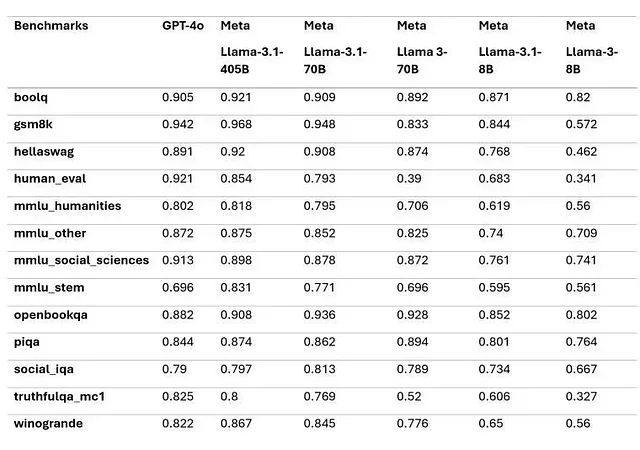
\includegraphics[width=0.8\textwidth]{medium_llama-gpt.png}
    \caption[13F voorbeeld 4]{\label{fig:gpt-versus-llama-benchmarks} Afbeelding toont een statistische vergelijking van GPT- en LlaMA-modellen op veelgebruikte NLP-benchmarks. \autocite{ResearchGRaph2024}}
\end{figure}

\subsection{Validatie van Large Language Models (LLMs) voor Gegevensextractie uit 13F-bestanden}

Volgens \autocite{Huang2024} zijn er bij de evaluatie van Large Language Models (LLMs) voor het extraheren van gegevens uit 13F-bestanden specifieke uitdagingen en metrieken die in overweging moeten worden genomen
In de bredere context van modelvalidatie, zoals besproken door \textcite{Islam2024}, zijn er verschillende technieken die kunnen worden aangepast om de prestaties van LLMs bij gegevensextractie uit 13F-bestanden te evalueren. Deze technieken variëren afhankelijk van de specifieke aspecten van het model en de aard van de data.

\subsubsection{Validatiemetrics en Uitdagingen}
\label{sec:LLMValidation}

\begin{enumerate}
    \item \textcite{Islam2024} benadrukt dat de nauwkeurigheid van een LLM bij het extraheren van specifieke gegevens zoals aandelenposities, waarden en data uit de complexe structuur van 13F-bestanden moet worden gemeten. Dit kan worden gedaan door de geëxtraheerde gegevens te vergelijken met een gecontroleerde dataset van handmatig gevalideerde informatie. Holdout Validation kan hier worden toegepast, waarbij het model wordt getraind op een deel van de data en getest op een ander deel om de nauwkeurigheid te evalueren.
    \item \textcite{Islam2024} geeft aan dat 13F-bestanden een strikte structuur en format hebben. Het is cruciaal om te controleren of de LLM in staat is om gegevens correct te interpreteren en om te zetten naar het gewenste formaat. Metrics zoals precisie en recall kunnen helpen bij het beoordelen van hoe goed de LLM voldoet aan de specificaties van het document. Hier kunnen de F1 Score en Cross-Validation nuttig zijn om een gebalanceerd beeld te krijgen van het model's prestaties over verschillende datasplitsingen.
    \item \textcite{Islam2024} merkt op dat de validatie ook de robuustheid van het model onder verschillende omstandigheden moet testen. Dit houdt in dat de LLM moet presteren bij variaties in de indeling van 13F-bestanden, of bij fouten en inconsistenties in de gegevens. Adversarial Testing kan hierbij worden ingezet om specifieke zwakheden in het model bloot te leggen.
    \item \textcite{Islam2024} wijst erop dat naast nauwkeurigheid, de snelheid waarmee een LLM gegevens kan extraheren ook belangrijk is. Evalueren hoe snel en efficiënt een model grote hoeveelheden 13F-bestanden kan verwerken, is cruciaal voor praktische toepassingen. Human Evaluation kan nuttig zijn om niet alleen de snelheid, maar ook de praktische bruikbaarheid en de outputkwaliteit van het model te beoordelen.
\end{enumerate}

\subsubsection{Best Practices voor Evaluatie}

\begin{enumerate}
    \item \textcite{Huang2024} beveelt het gebruik van een gouden dataset aan, bestaande uit 13F-bestanden met handmatig gevalideerde gegevens, om de prestaties van de LLM te meten. Deze dataset moet divers en representatief zijn voor de variaties in 13F-bestanden. Het gebruik van Zero-shot Evaluation kan helpen om het vermogen van het model te beoordelen om goed te presteren op onverwachte varianten binnen deze dataset.
    \item \textcite{Islam2024} stelt voor om een iteratief evaluatieproces te implementeren waarbij feedback van eerdere evaluaties wordt gebruikt om het model verder te verfijnen. Dit helpt bij het verbeteren van de nauwkeurigheid en robuustheid van het model. Cross-Validation kan hier opnieuw nuttig zijn om het model te blijven testen tijdens het verfijningsproces.
    \item \textcite{Islam2024} suggereert dat offline evaluaties, zoals het testen van het model op een vaste dataset, gecombineerd moeten worden met online evaluaties door het model te testen op echte gegevensstromen. Dit biedt een uitgebreide beoordeling van zowel de theoretische als praktische prestaties van de LLM. Perplexity kan hierbij worden gebruikt om de voorspellende kwaliteit van het model in online settings te meten.
\end{enumerate}
Door deze benaderingen en metrics te integreren in het validatieproces, kan er een effectieve en betrouwbare LLM ontwikkeld worden voor het extraheren van gegevens uit 13F-bestanden, waardoor de nauwkeurigheid en efficiëntie van de gegevensverwerking verbeterd.




\paragraph{Conclusie}

Samengevat is GPT een geavanceerde, commercieel verkrijgbare optie voor sommige NLP-taken, terwijl LLaMA een praktisch open-source alternatief is, vooral wanneer financiële beperkingen of de behoefte aan personalisatie van het grootste belang zijn. Door zorgvuldige selectie, training en finetuning van LLaMA-modellen kunnen betrouwbare, op maat gemaakte resultaten worden verkregen voor gerichte toepassingen, zonder de kosten van betalende modellen zoals GPT4o.\\
Dus wordt voor dit onderzoek Llama geselecteerd om de POC te ontwikkelen.

\subsection{Data vereisten voor LLMs te trainen}
\label{sec:DataVereisten}
Volgens \textcite{Scispace} is er minstens 0.5\% van de originele dataset nodig om een LLM effectief te trainen. Dit minimale percentage kan leiden tot verbeterde prestaties, waarbij modellen, ondanks het gebruik van een fractie van de data, een aanzienlijke nauwkeurigheid behalen in specifieke taken.









% ----------------------------------------------------------------------------
\section{Technieken en Tools}
\subsection{SpaCy versus NLTK}

De volgende tabel geeft een vergelijkende analyse van SpaCy en NLTK op basis van belangrijke functies die relevant zijn voor tekstsamenvatting.


\begin{table}[H]
    \centering
    \begin{tabular}{|p{4cm}|p{5cm}|p{5cm}|}
        \hline
        \textbf{Functie} & \textbf{NLTK} & \textbf{SpaCy} \\ \hline
        \textbf{01. Precisie} & 0.51 & 0.72 \\ \hline
        \textbf{02. Recall} & 0.65 & 0.65 \\ \hline
        \textbf{03. F-Score} & 0.58 & 0.69 \\ \hline
        \textbf{04. Tokenisatiesnelheid} & 4 ms & 0.2 ms \\ \hline
        \textbf{05. Taggingsnelheid} & 443 ms & 1 ms \\ \hline
        \textbf{06. Ondersteuning voor Classificatie} & Ja & Ja \\ \hline
        \textbf{07. Onderwerpmodellering} & Nee & Ja \\ \hline
        \textbf{08. Vectorisatie} & Nee & Ja \\ \hline
        \textbf{09. Ondersteunde Taalmodellen} & Basis Tokenizatie en parsing & Geavanceerde modellen met voorgetrainde vectors \\ \hline
        \textbf{10. Grootte en Afhankelijkheden van de Bibliotheek} & Lichtgewicht, minimale afhankelijkheden & Zwaarder, meer afhankelijkheden door geavanceerde functies \\ \hline
    \end{tabular}
    \caption{Vergelijkende Analyse van SpaCy en NLTK \autocite{amade2024automatic}}
    \label{tab:Vergelijking Spacy en NLTK}
\end{table}


Here are some examples demonstrating the strengths of SpaCy over NLTK:

\paragraph{Prestatiewaarden (Precisie, Recall, F-Score):} SpaCy behaalt een precisie van 0.72 en een F-Score van 0.69 bij het genereren van samenvattingen, terwijl NLTK respectievelijk 0.51 en 0.58 scoort. Dit wijst op een betere nauwkeurigheid en effectiviteit van SpaCy in vergelijking met NLTK.

\paragraph{Snelheid van Tokenizatie en Tagging:} Volgens \textcite{Saadani_2024} tokeniseert SpaCy tekst in 0,2 milliseconden, terwijl NLTK 4 milliseconden nodig heeft. Dit maakt SpaCy veel sneller en geschikter voor real-time toepassingen zoals chatbots en live datastreams.

\textbf{Tokenisatie} is het proces van het splitsen van tekst in kleinere eenheden, zoals woorden of zinnen, die "tokens" worden genoemd. Bijvoorbeeld, de zin "Het is een mooie dag" wordt getokeniseerd in de tokens: ["Het", "is", "een", "mooie", "dag"].

\textbf{Tagging} verwijst naar het toewijzen van labels of tags aan de getokeniseerde eenheden om hun grammaticale rol of betekenis te identificeren. Bijvoorbeeld, in de zin "Het is een mooie dag," zou tagging de woorden als volgt kunnen labelen: [("Het", B-ARTIKEL), ("is", B-WERKWOORD), ("een", B-ARTIKEL), ("mooie", B-BIJVOEGLIJK NAAMWOORD), ("dag", B-NAAMWOORD)].

\paragraph{Ondersteuning voor Geavanceerde NLP-functies:} \autocite{spacyff} biedt ingebouwde ondersteuning voor complexe NLP-functies zoals topic modellering en vectorisatie. NLTK vereist vaak extra maatwerk of externe bibliotheken voor deze functionaliteiten, wat SpaCy meer geschikt maakt voor geavanceerde machine learning taken.

\paragraph{Gebruiksvriendelijkheid:} \autocite{spacyff} heeft een intuïtieve API met uitgebreide documentatie en kant-en-klare modules, waardoor het gemakkelijker is om mee te werken. NLTK vereist vaak meer configuratie en maatwerk, wat de leercurve kan verhogen en de implementatietijd verlengt.

\paragraph{Conclusie}
Samenvattend, SpaCy is een krachtigere en efficiëntere tool voor tekstsamenvatting vanwege zijn hogere precisie, snelheid en ondersteuning voor geavanceerde NLP-functies. NLTK, hoewel veelzijdig, is beter geschikt voor taken of projecten die meer aanpassing vereisen. De keuze tussen deze tools hangt af van de specifieke eisen van het project, waaronder de complexiteit van de taak, de benodigde functies en de beschikbare middelen.


\subsection{Database Management Systemen (DBMS)}
In deze sectie gaat er bekeken worden welke databank gebruikt zal worden na het structuren en standaardiseren van de 13F-meldingen. Hier zal besproken worden of er SQL of nosql gebruikt zal worden vervolgens zal er een specifieke databank gekozen worden die aan ACID voldoet.

\subsubsection{ACID}
Volgens \autocite{Kaur2024} zijn de ACID-eigenschappen—Atomiciteit, Consistentie, Isolatie, en Duurzaamheid—zijn fundamenteel voor het waarborgen van betrouwbare transacties in een Database Management Systeem (DBMS). Hieronder volgt een korte uitleg van elke eigenschap:

\begin{enumerate}
    \item \textbf{Atomiciteit:} Atomiciteit zorgt ervoor dat een transactie wordt behandeld als één ondeelbare eenheid van werk. Dit betekent dat alle bewerkingen binnen de transactie volledig worden uitgevoerd of helemaal niet. Als een deel van de transactie mislukt, wordt de gehele transactie teruggedraaid naar de oorspronkelijke staat, waardoor dataconsistentie en integriteit worden gewaarborgd.
    
    \item \textbf{Consistentie:} Consistentie verzekert dat een transactie de database van een consistente staat naar een andere consistente staat brengt. De database moet zowel voor als na de transactie in een consistente toestand verkeren. Dit houdt in dat integriteitsregels, zoals unieke sleutels en vreemde sleutels, behouden blijven om dataconsistentie te waarborgen.
    
    \item \textbf{Isolatie:} Isolatie zorgt ervoor dat meerdere transacties gelijktijdig kunnen worden uitgevoerd zonder elkaar te beïnvloeden. Elke transactie moet geïsoleerd blijven van andere transacties totdat deze is voltooid. Deze isolatie voorkomt problemen zoals 'dirty reads', niet-herhaalbare leesacties, en 'phantom reads', wat bijdraagt aan de consistentie van de database.
    
    \item \textbf{Duurzaamheid:} Duurzaamheid garandeert dat zodra een transactie is vastgelegd, de resultaten permanent zijn en overleven ondanks eventuele systeemfouten. De wijzigingen die door de transactie zijn aangebracht, worden blijvend opgeslagen in de database en blijven intact, zelfs bij systeemcrashes.
\end{enumerate}

Deze eigenschappen vormen samen een kader voor het waarborgen van de consistentie, integriteit en betrouwbaarheid van gegevens in een DBMS. Ze zorgen ervoor dat transacties op een betrouwbare en consistente manier worden uitgevoerd, zelfs in het geval van systeemfouten, netwerkproblemen of andere complicaties. Dankzij de ACID-eigenschappen blijft een database een betrouwbaar en efficiënt hulpmiddel voor het beheren van gegevens in moderne organisaties.
\subsubsection{SQL versus NOSQL}
Bij het kiezen tussen SQL- en Nosql-databases is het belangrijk om de onderliggende architectuur en toepassingsmogelijkheden te begrijpen \autocite{khan2023performance}. SQL-databases zijn ontworpen voor het organiseren van gestructureerde data, waardoor ze ideaal zijn voor online transaction processing (OLTP). Ze presteren uitstekend in situaties waarin complexe query’s, consistentie en relationeel databeheer vereist zijn.NoSQL-databases ondersteunen horizontale schaalbaarheid en zijn geschikt voor het verwerken van grote hoeveelheden ongestructureerde data, waardoor ze ideaal zijn voor big data-analyse. De keuze tussen beide hangt grotendeels af van de specifieke behoeften van het onderzoek, zoals de focus op datastructuur of schaalbaarheid.

In dit onderzoek is gekozen voor een SQL-database. Deze keuze is gebaseerd op de noodzaak om gestructureerde data uit de 13F-meldingen te beheren, waarbij consistente gegevensintegriteit en de mogelijkheid om complexe query’s uit te voeren cruciaal zijn. SQL-databases bieden de benodigde functionaliteiten voor het beheer van relationele gegevens en het uitvoeren van geavanceerde analyses, wat essentieel is voor het succes van dit project \autocite{khan2023performance}.

\paragraph{SQL-databank}
Op basis van de gedetailleerde analyse die door \autocite{Javija2024} werd uitgevoerd is PostgreSQL gekozen voor dit proefschrift vanwege de geavanceerde functies, robuuste gegevensintegriteit en uitbreidbare architectuur. In tegenstelling tot andere SQL-databases, blinkt PostgreSQL uit in het verwerken van complexe datamanipulatie, het bieden van sterke ACID compliance en het ondersteunen van aangepaste datatypes en functies. Dit maakt PostgreSQL bijzonder geschikt voor bedrijfstoepassingen en datawarehousing waar schaalbaarheid en geavanceerd databeheer cruciaal zijn. Hoewel PostgreSQL een steilere leercurve heeft dan sommige alternatieven, maken de uitgebreide functie set en betrouwbaarheid het een optimale keuze om aan de complexe eisen van dit project te voldoen.
\subsection{Unsloth.AI}
Volgens \textcite{unsloth2024} is unsloth een platform dat zich richt op het verbeteren van de snelheid en efficiëntie van het trainen van grote taalmodellen (LLMs). Traditioneel gezien kunnen deze trainingsprocessen lang duren en veel geheugen vereisen, maar Unsloth heeft technologie ontwikkeld die dit proces tot 30 keer sneller maakt dan gebruikelijke methoden zoals Flash Attention 2 (FA2). Bovendien verbruikt Unsloth hierbij tot 90\% minder geheugen. Het platform werkt met verschillende soorten GPU's, waaronder die van NVIDIA, AMD en Intel, zonder dat er dure hardware-upgrades nodig zijn. Dit maakt het trainen van AI-modellen toegankelijker en goedkoper, met mogelijkheden variërend van gratis tot uitgebreide enterprise-oplossingen.


% ----------------------------------------------------------------------------

\section{Uitdagingen en beperkingen}
In dit hoofdstuk zullen enkele uitdagingen en beperkingen benoemt worden
\subsection{Variable structuur}
voor 2013 bevatten 13F-meldingen enigszins verschillende variabele structuren, maar deze variaties zijn belangrijk omdat ze het moeilijk maken om de gegevens te lezen en te analyseren. voor 2013 waren de 13F-meldingen variabeler in de manier waarop ze gegevens verstrekten, waardoor het moeilijk was om beleggingsportefeuilles door de tijd heen te vergelijken. Door dit gebrek aan standaardisatie moesten onderzoekers en analisten zorgvuldig omgaan met deze gegevens om consistente en nauwkeurige bevindingen te krijgen. Diepgaand onderzoek is nodig om interpretatiefouten te minimaliseren en investeringen en investeringspatronen als gevolg van verschillende rapportagestandaarden volledig te begrijpen.



\subsection{Databaseprestaties}
Uitdaging: Hoewel PostgreSQL goed presteert bij grote hoeveelheden gestructureerde data, kan het moeilijk zijn om de prestaties te optimaliseren naarmate de hoeveelheid data en het aantal gelijktijdige gebruikers toeneemt.

Beperking: Bij zeer grote datasets of een hoge mate van gelijktijdige toegang kunnen er prestatieproblemen optreden. Het kan nodig zijn om uitgebreide optimalisaties en schaalstrategieën te implementeren, zoals partitionering of het gebruik van read replicas.
% ----------------------------------------------------------------------------
\section{Tekortkomingen in huidig onderzoek}
Dit hoofdstuk geeft enkele tekortkomingen weer in het huidig onderzoek.

\paragraph{Beveiliging en Privacy}
Het beschermen van gevoelige financiële gegevens tegen ongeautoriseerde toegang en datalekken is complex en vereist naleving van privacywetgeving. Onvoldoende beveiliging kan leiden tot datalekken, verlies van vertrouwen en juridische problemen. Implementeer encryptie, toegangscontrole en regelmatige beveiligingsaudits om gegevens te beschermen. Zorg ervoor dat uw systemen voldoen aan relevante regelgeving en best practices voor gegevensbeveiliging.

\paragraph{Schaalbaarheid en Prestaties}
Groeiende hoeveelheden gegevens kunnen leiden tot prestatieproblemen bij opslag en analyse, wat complexe oplossingen vereist voor snelle toegang. Slechte prestaties kunnen vertragingen veroorzaken in rapportage en analyse, wat de besluitvorming en efficiëntie beïnvloedt. Gebruik schaalbare databases en technieken zoals gegevenspartitionering en caching. Monitor en optimaliseer regelmatig de prestaties om problemen te voorkomen.
